\pdfminorversion=7
\documentclass[12pt]{article}
\usepackage{fullpage}
\usepackage{cmu-techreport}
\usepackage{listings}
\usepackage{minted}
\usemintedstyle{borland}
\usepackage{xcolor}
\usepackage{graphicx}
\usepackage{lscape}
\usepackage{rotating}
\usepackage{booktabs}
\usepackage{multirow}
\usepackage{bigstrut}
\usepackage{dcolumn}

\definecolor{dkgreen}{rgb}{0,0.6,0}
\definecolor{gray}{rgb}{0.5,0.5,0.5}
\definecolor{mauve}{rgb}{0.58,0,0.82}

%\lstset{frame=tb,
%  language=Python,
%  aboveskip=3mm,
%  belowskip=3mm,
%  showstringspaces=false,
%  columns=flexible,
%  basicstyle={\small\ttfamily},
%  numbers=none,
%  numberstyle=\tiny,
%  keywordstyle=,
%  commentstyle=\color{dkgreen},
%  stringstyle=\color{mauve},
%  breaklines=true,
%  breakatwhitespace=true,
%  tabsize=3
%}

\lstset{language=Python, 
  breaklines=true,  
  basicstyle=\ttfamily\bfseries,
  columns=fixed,
  keepspaces=true,
  identifierstyle=\color{blue}\ttfamily,
  keywordstyle=\color{cyan}\ttfamily,
  stringstyle=\color{purple}\ttfamily,
  commentstyle=\color{green}\ttfamily,
  } 


\title{STAT 608 Homework \#9}
\author{E. Lee Rainwater}
\date{22 July 2020}
\abstract{Topic analysis was performed upon a dataset of complaints from Honda and Acura owners filed to the National Highway Transportation Safety Administration with the goal of correlating text clusters of complaint characteristics with whether the vehicle was involved in a crash.}

%\keywords{technical reports, typesetting, Carnegie Mellon University}

%\trnumber{CMU-CS-90-999}

%\citationinfo{\begin{center}
%To appear in a \TeX\ collection near you.
%\end{center}}

%\arpasupport{fox}
% \othersupport{the National Science Foundation under grant number 99-999-99}
% \authorsupport{The author holds a Froboz Gradual Fellowship.}

% \otherdisclaimer{NSF}



\makeatother

\usepackage{listings}
\renewcommand{\lstlistingname}{Listing}

\begin{document}
\maketitle

\section{Introduction}
In this exercise, the scikit-learn library of Python was utilized to generate a total of 8 text clusters (topic groups) from the descriptive text of complaints lodged by, or on behalf of, owners of Honda and Acura automobiles. The dataset contained 5,330 records, of which 571 were flagged as involving a traffic accident. These records were processed utilizing a TF-IDF \textit{Text Frequency-Inverse Document Frequency} algorithm vectorizes words, filters out stop words, equivalences synonymic expressions, then finally computes \textit{term frequency} and \textit{inverse term frequency} values for each word in the corpus.


The following general steps were used to generate topic groups and associate each record with its corresponding group: 
\begin{enumerate}
\item Read the data contained in  \texttt{HondaComplaints.xlsx} into a Pandas dataframe
\item Identify any truncated records
\item Set up a dictionary of synonyms and a list of stop words
\item Use scikit-learn's \texttt{CountVectorizer} to vectorize the collection of records into a matrix of token counts
\item Via scikit-learn's \texttt{TfidfTransformer}, transform the token count matrix into a term-frequency matrix and report frequencies of the most and least common terms
\item Decompose the term-frequency matrix to generate topic groups and assign each original record to its corresponding topic group
\item Convert the resulting array into a dataframe and append it to the original dataframe. This dataframe is then stored as a \texttt{Pickle} document.
\end{enumerate}

The resulting topic group information was then processed by a second Python script to train a series of models to classify whether the vehicle associated with a complaint was involved in an accident, based upon the verbiage in the description. The Python script implemented this general process:
\begin{enumerate}
\item Read the \texttt{Pickle} file generated by the previous script into a Pandas dataframe \textit{hence termed the ``model dataset''}
\item Replace and impute any missing data or outliers, and 1-hot encode any nominal or binary variables
\item A DEAP \texttt{eaSimple} evolutionary algorithm is used to select features which, when fitted with a logistic regression, will minimize the resulting BIC \textit{Bayesian Information Criterion}.
\item A logistic regression of the selected features is applied to a 70/30 training/validation partition of the model dataset
\item A logistic regression with stepwise feature selection is performed, and likewise subjected to a 70/30 validation
\item A decision tree classification is performed of the model dataset. Hyperparameter optimization is accomplished by iterating the model over a list of pre-selected maximum depths. The model is subjected to 5-fold cross-validation.
\item A random forest classification is performed of the model dataset, with the maximum tree depth likewise optimized by iterating of a list of pre-selected values. Again, this model is subjected to 5-fold cross-validation.
\end{enumerate}
These models are compared on the basis of average squared error (ASE)


\section{General Observations}
The initial creation of topic groups was an iterative process. As topic groups were generated, words were found that did not contribute substantially to the context of the group. Such words were added to the \textit{stop word} list. Some words were also found that were semantically equivalent to others; these were added to a synonym dictionary.

\begin{table}
\caption{List of Stop Words}
\label{tab:stopWords}
{\footnotesize
\begin{lstlisting}
sw = ['tl', 'tr', 'jb', 'xxx', 'know', 'thing', 'regard', 'provide',
      'car','honda', 'notified', 'acura', 'call', 'tell', 'approximately',
      'read', 'sinc', 'id', 'offer', 'nhtsa', 'unit', 'go', 'many', 'need',
      'make', 'number', 'information', 'cause', 'receive', 'prior', 
      'notice', 'approximate', 'told', 'entire', 'happen',
      'dealer', 'problem', 'contact', 'internet', 'appear', 'year',
      'online', 'find', 'lj', 'responsible', 'consumer', 'part', 'van']
\end{lstlisting}
}
\end{table}

\begin{table}
\caption{Synonym Dictionary}
\label{tab:synDict}
{\footnotesize
\begin{lstlisting}
syn = {"automobile": 'car', 
        "vehicle": 'car', 
        "gasoline": 'gas', 
        "crv" : 'cr-v',
        "cr v": 'cr-v',
        "cr": 'cr-v',
        "fix": 'repair',
        "dealership": 'dealer',
        "honda dealer": 'dealer',
        "manufacturer": 'honda', 
        "replacement":'replace',
        "suddenly": 'sudden',
        "recall campaign":'recall',
        "campaign": 'recall',
        "issue": 'problem',
        "complaint":'problem',
        "highway": 'road', 
        "seat belt":'seatbelt',
        "air bag":'airbag',
        "air  bag":'airbag',
        "airbags": 'airbag',
        "srs":'airbag',
        "sr": 'airbag',
        "bag":'airbag'}
\end{lstlisting}
}
\end{table}

The most common terms, after filtering stop words and mapping synonyms, are depicted in Figure~\ref{fig:termFreq}.
\begin{figure}
	\begin{center}
	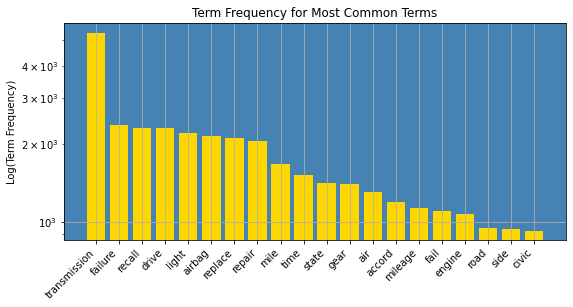
\includegraphics[width=\textwidth, keepaspectratio, angle=0]{termFreq.png}
	\caption{Frequency of Common Terms}
	\label{fig:termFreq}
	\end{center}
\end{figure}

\subsection{Final Clusters and Characteristics}
The final clusters are presented in the Appendix. While further refinement of stop words would be possible, by this point Topic \#7, shown in Table~\ref{tab:cluster}, has emerged as being a probable identifier of vehicular accidents.


\begin{table}
\caption{Topic \#7---A Likely Identifer of Crashes}
\label{tab:cluster}
{\footnotesize
\begin{lstlisting}
Topic #7: 
+airbag        +air           +seat          +side          +driver        
+bag           +deploy        +passenger     +belt          +light         
+front         +injury        +recall        +accident      +crash         
\end{lstlisting}
}
\end{table}


\section{Classification Models}
The various classification models that were utilized to form predictors of crashes are summarized in Table~\ref{tab:modelComp} and presented in greater detail in the Appendix. For the \textit{decision tree} and \textit{random forest} models, hyperparameters were optimized via a grid search through a list of maximum tree depths from 5 through 20, with the model with the best \textit{f1} value retained for inclusion in the ensemble model. The \textit{genetic algorithm} model is inherently self-optimizing, apart from adjusting the number of generations. In this case, the genetic algorithm selected nine features by iteration \#18, as shown in Figure~\ref{fig:featureSelect}. Each of the four models detected \texttt{prob7} (Topic \#7) as the most significant predictor of the target variable, \texttt{crash}. Of these models, the random forest with 5-fold cross-validation produced the best validation fit, with the lowest \textit{Mean Square Error} as well as the lowest misclassification rate.

% Table generated by Excel2LaTeX from sheet 'Sheet1'
\begin{table}[htbp]
  \centering
  \caption{Model Comparison}
    \begin{tabular}{lrrlr}
    \textit{Algorithm} & \multicolumn{1}{l}{\textit{MISC}} & \multicolumn{1}{l}{\textit{MSE}} & \textit{Hyperparam.} & \multicolumn{1}{l}{\textit{Opt. Value}} \bigstrut[b]\\
    \hline
    GA with Logistic Regression & 9.20\% & 0.0660 & No. Gens & 25 \bigstrut[t]\\
    Logistic Regression with Stepwise & 9.40\% & 0.0659 & n/a   & n/a \\
    DT with 5-fold Cross-Validation & 4.90\% & 0.0391 & Tree Depth & 6 \\
    RF with 5-fold Cross-Validation & 4.00\% & 0.0284 & Forest Depth & 13 \\
    \hline
    \end{tabular}%
  \label{tab:modelComp}%
\end{table}%

\begin{figure}
	\begin{center}
	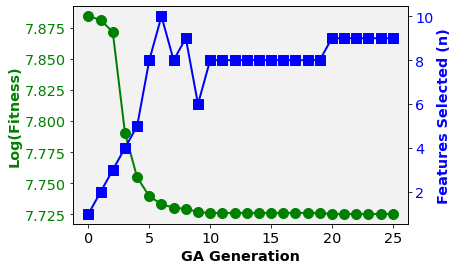
\includegraphics[width=\textwidth, keepaspectratio, angle=0]{featureSelect.png}
	\caption{Genetic Feature Selection}
	\label{fig:featureSelect}
	\end{center}
\end{figure}



\section{Ensemble Model}
The four optimized models are combined into an ensemble model utilizing the \texttt{scikit-learn VotingClassifier}. This classifier compares the class label that represents the mode for each model, and selects the class for that sample based upon a majority vote. Weights can be passed into the method to enforce model preference. However, no weights were specified in the case of this exercise, so each model is given equal weight in determining the selected class. Assessment of the four models with 5-fold cross-validation is shown in Table~\ref{tab:ensModel}.

\begin{center}
\begin{table}[H]
\caption{Ensemble Model Evaluation Output}
\begin{verbatim}
Accuracy: 0.89 (+/- 0.00) [GA Logistic Regression]
Accuracy: 0.89 (+/- 0.00) [SW Logistic Regression]
Accuracy: 0.92 (+/- 0.01) [Decision Tree]
Accuracy: 0.89 (+/- 0.00) [Random Forest]
Accuracy: 0.93 (+/- 0.01) [Ensemble]
\end{verbatim}
\label{tab:ensModel}
\end{table}
\end{center}

The ensemble model produced slightly greater classification accuracy than the Decision Tree model, at 93\% vs 92\%.

\section{Opportunities for Improvement}
Python's \texttt{nltk} (Natural Language Tool Kit) library provides a standard list of English stop words which may be useful for filtering words that add no semantic meaning to the text. This, when used in conjunction with the user-supplied stop word list, could improve the quality and relevancy of the topic clusters.
The logistic regression models could possibly be improved by utilizing algorithms that allow regularization. This could reduce some of the overfitting that is evident.

\section{Conclusion}
The furnished NHTSA dataset was textually analyzed for topic groups, with machine learning models applied to the resulting groups to determine which review groups were indicative of the subject vehicle having been involved in a collision. As stated previously, the ensemble model produces the highest accuracy (93\%) in identifying descriptions associated with a vehicular accident. The ensemble model which effectively combines the results of the  four non-ensemble models.  Of the individual models, the decision tree model had the highest overall accuracy, 93\%.
\pagebreak
\section{Appendix}




\subsection{Topic Clusters}
Below are the topic clusters generated by TF-IDF.

{\footnotesize
\begin{lstlisting}
*---------------       STARTING TERM-FREQUENCY MATRIX     ---------------*
*---------------           DECOMPOSITION USING LDA        ---------------*
*---------------  IDENTIFYING TOPIC CLUSTERS USING TFIDF  ---------------*
*---------------              GENERATED TOPICS            ---------------*
*------------------------------------------------------------------------*
Topic #1: 
+door          +headlight     +beam          +low           +open          
+switch        +rust          +burn          +fire          +window        
+com           +smell         +area          +wire          +close         

Topic #2: 
+recall        +ignition      +key           +please        +break         
+frame         +accord        +compressor    +system        +electrical    
+turn          +subframe      +dashboard     +switch        +ac            

Topic #3: 
+service       +noise         +brake         +already       +replace       
+like          +even          +loud          +though        +still         
+repair        +refuse        +see           +one           +sound         

Topic #4: 
+transmission  +mile          +warranty      +new           +replace       
+pay           +time          +start         +buy           +cost          
+gear          +back          +work          +day           +home          

Topic #5: 
+transmission  +recall        +light         +failure       +repair        
+gear          +replace       +engine        +accord        +state         
+check         +jerk          +mileage       +shift         +slip          

Topic #6: 
+tire          +road          +oil           +right         +lane          
+freeway       +front         +leave         +away          +traffic       
+drive         +leak          +major         +wheel         +accident      

Topic #7: 
+airbag        +air           +seat          +side          +driver        
+bag           +deploy        +passenger     +belt          +light         
+front         +injury        +recall        +accident      +crash         

Topic #8: 
+failure       +drive         +mileage       +stop          +brake         
+accelerate    +mph           +state         +update        +engine        
+current       +park          +speed         +move          +pedal         
\end{lstlisting}
}
\pagebreak


\subsection{Feature Importance Plots}
\begin{figure}[H]
	\begin{center}
	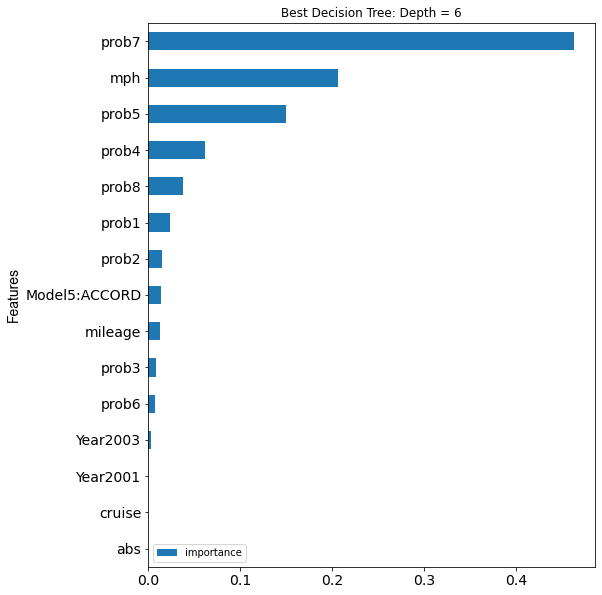
\includegraphics[width=\textwidth, keepaspectratio, angle=0]{DT_FeatureImp.png}
	\caption{Decision Tree Feature Importance}
	\label{fig:DT_FeatureImp}
	\end{center}
\end{figure}

\begin{figure}[H]
	\begin{center}
	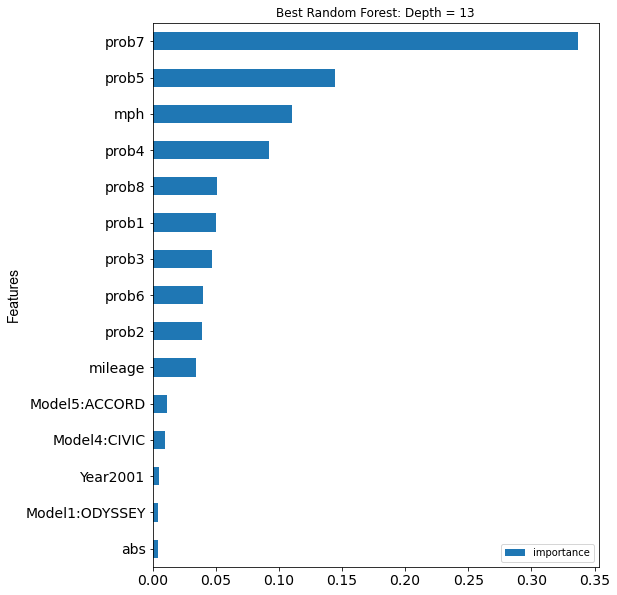
\includegraphics[width=\textwidth, keepaspectratio, angle=0]{RF_FeatureImp.png}
	\caption{Random Forest Feature Importance}
	\label{fig:RF_FeatureImp}
	\end{center}
\end{figure}

\pagebreak
\subsubsection{Model Code Output}
\begin{verbatim}
********** Data Preprocessing ***********
Features Dictionary Contains:
10 Interval, 
3 Binary, 
3 Nominal, and 
3 Excluded Attribute(s).

Data contains 5330 observations & 19 columns.


Attribute Counts
.................. Missing  Outliers
NhtsaID......         0         0
Year.........         0         0
Make.........         0         0
Model........         0         0
State........         0         0
description..         0         0
crash........         0         0
mph..........         0         1
abs..........         0         0
mileage......         1        70
cruise.......         0         0
prob1........         0         0
prob2........         0         0
prob3........         0         0
prob4........         0         0
prob5........         0         0
prob6........         0         0
prob7........         0         0
prob8........         0         0

*-----------------------------------------------------------------------------*
*-------------    GA Selection using   bic Fitness           -----------------*
*-------------    sklearn Models and   star Initialization   -----------------*

 
gen	nevals	features	range  	min    	avg    	max    	Ln(Fit)
0  	24    	1       	4751.05	2655.06	3739.01	7406.11	7.88422
1  	24    	2       	4758.83	2647.28	4062.25	7406.11	7.88129
2  	22    	3       	755.323	2621.64	2761.54	3376.97	7.87156
3  	23    	4       	245.55 	2417.62	2622.1 	2663.17	7.79054
4  	23    	5       	330.37 	2332.8 	2545.01	2663.17	7.75483
5  	23    	8       	334.388	2297.55	2426.36	2631.94	7.7396 
6  	23    	10      	1799.85	2282.94	2414.6 	4082.78	7.73322
7  	22    	8       	55.9   	2276.5 	2292.19	2332.4 	7.73039
8  	24    	9       	42.279 	2274.46	2281.78	2316.74	7.7295 
9  	22    	6       	28.178 	2268.59	2276.57	2296.77	7.72691
10 	24    	8       	1832.72	2266.93	2360.39	4099.66	7.72618
11 	21    	8       	301.75 	2266.93	2290.13	2568.68	7.72618
12 	21    	8       	26.135 	2266.93	2268.71	2293.07	7.72618
13 	22    	8       	26.135 	2266.93	2268.42	2293.07	7.72618
14 	24    	8       	234.775	2266.93	2277.46	2501.71	7.72618
15 	23    	8       	234.775	2266.93	2279.45	2501.71	7.72618
16 	23    	8       	225.223	2266.93	2279.4 	2492.16	7.72618
17 	24    	8       	234.775	2266.93	2290.23	2501.71	7.72618
18 	24    	8       	8.529  	2266.93	2267.86	2275.46	7.72618
19 	24    	8       	226.302	2266.93	2278.5 	2493.24	7.72618
20 	18    	9       	2.682  	2265.16	2266.9 	2267.84	7.7254 
21 	22    	9       	9.516  	2265.16	2267.94	2274.67	7.7254 
22 	24    	9       	17.387 	2265.16	2267.65	2282.54	7.7254 
23 	23    	9       	229.318	2265.16	2284.21	2494.48	7.7254 
24 	24    	9       	302.695	2265.16	2281.44	2567.85	7.7254 
25 	22    	9       	59.093 	2265.16	2268.05	2324.25	7.7254 
GA Runtime  41.44947409629822  sec.
Individuals in HoF:  146
*-----------------------------------------------------------------------------*
*------------------------   GA SELECTION BEST FEATURES   ---------------------*
*------------------------ Best Fitness      .. 2265.1572 ---------------------*
*------------------------ Features Selected .......... 9 ---------------------*

Optimization terminated successfully.
         Current function value: 0.203636
         Iterations 9

*=============================================================================*
AICC .......... 2192.814   AIC ........... 2192.765   BIC ............2265.157

                           Logit Regression Results                           
==============================================================================
Dep. Variable:                  crash   No. Observations:                 5330
Model:                          Logit   Df Residuals:                     5320
Method:                           MLE   Df Model:                            9
Date:                Thu, 23 Jul 2020   Pseudo R-squ.:                  0.4019
Time:                        10:51:25   Log-Likelihood:                -1085.4
converged:                       True   LL-Null:                       -1814.7
Covariance Type:            nonrobust   LLR p-value:                1.632e-308
=================================================================================
                    coef    std err          z      P>|z|      [0.025      0.975]
---------------------------------------------------------------------------------
const            -2.8601      0.258    -11.087      0.000      -3.366      -2.355
mph               0.0201      0.003      5.940      0.000       0.013       0.027
prob1            -3.0492      0.630     -4.837      0.000      -4.285      -1.814
prob3            -1.5235      0.494     -3.081      0.002      -2.493      -0.554
prob4            -3.4502      0.456     -7.569      0.000      -4.344      -2.557
prob5            -7.6413      0.644    -11.861      0.000      -8.904      -6.379
prob7             3.5171      0.261     13.452      0.000       3.005       4.030
prob8             0.8798      0.279      3.153      0.002       0.333       1.427
Model4:CIVIC      0.4620      0.144      3.199      0.001       0.179       0.745
Model5:ACCORD     0.6327      0.147      4.310      0.000       0.345       0.920
=================================================================================

Model Metrics
Observations...............      5330
Coefficients...............        10
DF Error...................      5320
Iterations.................       100
Mean Absolute Error........    0.1203
Avg Squared Error..........    0.0601
Accuracy...................    0.9161
Precision..................    0.6640
Recall (Sensitivity).......    0.4396
RSpecificity...............    0.9733
F1-Score...................    0.5290
Total Misclassifications...       447
MISC (Misclassification)...      8.4%
     class 0                     2.7%
     class 1                    56.0%


     Confusion     Class     Class
       Matrix          0         1
  Class 0.....      4632       127
  Class 1.....       320       251

*=============================================================================*
*------------------------ GA SELECTION 70/30 VALIDATION ----------------------*


Model Metrics..........       Training     Validation
Observations...........           3730           1600
Coefficients...........             10             10
DF Error...............           3720           1590
Iterations.............            100            100
Mean Absolute Error....         0.1149         0.1263
Avg Squared Error......         0.0577         0.0660
Accuracy...............         0.9225         0.9081
Precision..................     0.6908         0.6336
Recall (Sensitivity).......     0.4653         0.4560
Specificity................     0.9758         0.9661
F1-score...................     0.5561         0.5304
Total Misclassifications...        289            147
MISC (Misclassification)...       7.7%           9.2%
     class 0...............       2.4%           3.4%
     class 1...............      53.5%          54.4%


Training                  Class     Class
Confusion Matrix              0         1
Class 0..............      3260        81
Class 1..............       208       181


Validation                Class     Class
Confusion Matrix              0         1
Class 0..............      1370        48

C:\Users\rainwater-e\miniconda3\envs\cuda\lib\site-packages\sklearn\linear_model\
_logistic.py:764: ConvergenceWarning: lbfgs failed to converge (status=1):
STOP: TOTAL NO. of ITERATIONS REACHED LIMIT.

Increase the number of iterations (max_iter) or scale the data as shown in:
    https://scikit-learn.org/stable/modules/preprocessing.html
Please also refer to the documentation for alternative solver options:
    https://scikit-learn.org/stable/modules/linear_model.html#logistic-regression
  extra_warning_msg=_LOGISTIC_SOLVER_CONVERGENCE_MSG)
C:\Users\rainwater-e\miniconda3\envs\cuda\lib\site-packages\sklearn\linear_model\
_logistic.py:764: ConvergenceWarning: lbfgs failed to converge (status=1):
STOP: TOTAL NO. of ITERATIONS REACHED LIMIT.

Increase the number of iterations (max_iter) or scale the data as shown in:
    https://scikit-learn.org/stable/modules/preprocessing.html
Please also refer to the documentation for alternative solver options:
    https://scikit-learn.org/stable/modules/linear_model.html#logistic-regression
  extra_warning_msg=_LOGISTIC_SOLVER_CONVERGENCE_MSG)

Class 1..............        99        83

**********************************************************************
************* Logistic Regression with Stepwise Selection ************
**********************************************************************
Add  prob7                          with p-value 4.6029e-180
Add  prob8                          with p-value 1.45224e-34
Add  prob5                          with p-value 5.07763e-26
Add  prob4                          with p-value 3.3896e-09
Add  mph                            with p-value 1.39228e-08
Add  prob1                          with p-value 2.6664e-06
Add  Model2:CR-V                    with p-value 0.00144006
Add  prob3                          with p-value 0.00126067
Add  Model1:ODYSSEY                 with p-value 0.00177204
Add  cruise                         with p-value 0.0465067
Optimization terminated successfully.
         Current function value: 0.203005
         Iterations 9

*=============================================================================*
AICC .......... 2188.097   AIC ........... 2188.038   BIC ............2267.011

                           Logit Regression Results                           
==============================================================================
Dep. Variable:                  crash   No. Observations:                 5330
Model:                          Logit   Df Residuals:                     5319
Method:                           MLE   Df Model:                           10
Date:                Thu, 23 Jul 2020   Pseudo R-squ.:                  0.4038
Time:                        10:51:27   Log-Likelihood:                -1082.0
converged:                       True   LL-Null:                       -1814.7
Covariance Type:            nonrobust   LLR p-value:                7.536e-309
==================================================================================
                     coef    std err          z      P>|z|      [0.025      0.975]
----------------------------------------------------------------------------------
const             -2.3992      0.236    -10.178      0.000      -2.861      -1.937
prob7              3.5871      0.262     13.671      0.000       3.073       4.101
prob8              0.8646      0.279      3.099      0.002       0.318       1.412
prob5             -7.5779      0.644    -11.769      0.000      -8.840      -6.316
prob4             -3.4618      0.456     -7.592      0.000      -4.355      -2.568
mph                0.0188      0.003      5.678      0.000       0.012       0.025
prob1             -2.9902      0.625     -4.786      0.000      -4.215      -1.766
Model2:CR-V       -0.7040      0.200     -3.525      0.000      -1.096      -0.313
prob3             -1.6335      0.496     -3.295      0.001      -2.605      -0.662
Model1:ODYSSEY    -0.6756      0.213     -3.166      0.002      -1.094      -0.257
cruise             0.2340      0.118      1.991      0.047       0.004       0.464
==================================================================================

Model Metrics
Observations...............      5330
Coefficients...............        11
DF Error...................      5319
Iterations.................       100
Mean Absolute Error........    0.1191
Avg Squared Error..........    0.0600
Accuracy...................    0.9174
Precision..................    0.6710
Recall (Sensitivity).......    0.4501
RSpecificity...............    0.9735
F1-Score...................    0.5388
Total Misclassifications...       440
MISC (Misclassification)...      8.3%
     class 0                     2.6%
     class 1                    55.0%


     Confusion     Class     Class
       Matrix          0         1
  Class 0.....      4633       126
  Class 1.....       314       257


**********************************************************************
********************** Stepwise 70/30 Validation *********************
**********************************************************************


Model Metrics..........       Training     Validation
Observations...........           3730           1600
Coefficients...........             11             11
DF Error...............           3719           1589
Iterations.............            100            100
Mean Absolute Error....         0.1140         0.1251
Avg Squared Error......         0.0578         0.0659
Accuracy...............         0.9214         0.9062
Precision..................     0.6846         0.6212
Recall (Sensitivity).......     0.4576         0.4505
Specificity................     0.9755         0.9647
F1-score...................     0.5485         0.5223
Total Misclassifications...        293            150
MISC (Misclassification)...       7.9%           9.4%
     class 0...............       2.5%           3.5%
     class 1...............      54.2%          54.9%


Training                  Class     Class
Confusion Matrix              0         1
Class 0..............      3259        82
Class 1..............       211       178


Validation                Class     Class
Confusion Matrix              0         1
Class 0..............      1368        50
Class 1..............       100        82

**********************************************************************
***************** Decision Tree with Cross Validation ****************
**********************************************************************

Tree Depth:  5
C:\Users\rainwater-e\miniconda3\envs\cuda\lib\site-packages\sklearn\linear_model\
_logistic.py:764: ConvergenceWarning: lbfgs failed to converge (status=1):
STOP: TOTAL NO. of ITERATIONS REACHED LIMIT.

Increase the number of iterations (max_iter) or scale the data as shown in:
    https://scikit-learn.org/stable/modules/preprocessing.html
Please also refer to the documentation for alternative solver options:
    https://scikit-learn.org/stable/modules/linear_model.html#logistic-regression
  extra_warning_msg=_LOGISTIC_SOLVER_CONVERGENCE_MSG)
C:\Users\rainwater-e\miniconda3\envs\cuda\lib\site-packages\sklearn\linear_model\
_logistic.py:764: ConvergenceWarning: lbfgs failed to converge (status=1):
STOP: TOTAL NO. of ITERATIONS REACHED LIMIT.

Increase the number of iterations (max_iter) or scale the data as shown in:
    https://scikit-learn.org/stable/modules/preprocessing.html
Please also refer to the documentation for alternative solver options:
    https://scikit-learn.org/stable/modules/linear_model.html#logistic-regression
  extra_warning_msg=_LOGISTIC_SOLVER_CONVERGENCE_MSG)
Metric............  Mean    Std. Dev.
precision_macro... 0.8357    0.0485
recall_macro...... 0.7625    0.0329
f1_macro.......... 0.7888    0.0220

Tree Depth:  6
Metric............  Mean    Std. Dev.
precision_macro... 0.8278    0.0483
recall_macro...... 0.7777    0.0228
f1_macro.......... 0.7962    0.0169

Tree Depth:  7
Metric............  Mean    Std. Dev.
precision_macro... 0.8223    0.0546
recall_macro...... 0.7638    0.0157
f1_macro.......... 0.7854    0.0193

Tree Depth:  8
Metric............  Mean    Std. Dev.
precision_macro... 0.8135    0.0580
recall_macro...... 0.7570    0.0173
f1_macro.......... 0.7787    0.0264

Tree Depth:  9
Metric............  Mean    Std. Dev.
precision_macro... 0.8042    0.0519
recall_macro...... 0.7589    0.0210
f1_macro.......... 0.7760    0.0251

Tree Depth:  10
Metric............  Mean    Std. Dev.
precision_macro... 0.8118    0.0498
recall_macro...... 0.7659    0.0172
f1_macro.......... 0.7837    0.0225

Tree Depth:  11
Metric............  Mean    Std. Dev.
precision_macro... 0.8019    0.0542
recall_macro...... 0.7617    0.0204
f1_macro.......... 0.7767    0.0265

Tree Depth:  12
Metric............  Mean    Std. Dev.
precision_macro... 0.8000    0.0623
recall_macro...... 0.7680    0.0119
f1_macro.......... 0.7791    0.0291

Tree Depth:  13
Metric............  Mean    Std. Dev.
precision_macro... 0.8008    0.0511
recall_macro...... 0.7607    0.0173
f1_macro.......... 0.7756    0.0219

Tree Depth:  14
Metric............  Mean    Std. Dev.
precision_macro... 0.8028    0.0559
recall_macro...... 0.7665    0.0111
f1_macro.......... 0.7797    0.0235

Tree Depth:  15
Metric............  Mean    Std. Dev.
precision_macro... 0.8046    0.0561
recall_macro...... 0.7653    0.0179
f1_macro.......... 0.7801    0.0273

Tree Depth:  20
Metric............  Mean    Std. Dev.
precision_macro... 0.8046    0.0561
recall_macro...... 0.7653    0.0179
f1_macro.......... 0.7801    0.0273

Best Tree Depth:  6

FEATURE........... IMPORTANCE
prob7.............   0.4622
mph...............   0.2064
prob5.............   0.1500
prob4.............   0.0613
prob8.............   0.0373
prob1.............   0.0235
prob2.............   0.0145
Model5:ACCORD.....   0.0139
mileage...........   0.0130
prob3.............   0.0077
prob6.............   0.0074
Year2003..........   0.0028
abs...............   0.0000
cruise............   0.0000
Year2001..........   0.0000


Feature Importances:
<Figure size 432x288 with 0 Axes>
<Figure size 432x288 with 0 Axes>

Model Metrics
Observations...............      5330
Features...................        23
Maximum Tree Depth.........         6
Minimum Leaf Size..........         5
Minimum split Size.........         5
Mean Absolute Error........    0.0781
Avg Squared Error..........    0.0391
Accuracy...................    0.9507
Precision..................    0.8484
Recall (Sensitivity).......    0.6567
Specificity................    0.9859
F1-Score...................    0.7404
Total Misclassifications...       263
MISC (Misclassification)...      4.9%
     class 0                     1.4%
     class 1                    34.3%


     Confusion     Class     Class
       Matrix          0         1
  Class 0.....      4692        67
  Class 1.....       196       375


**********************************************************************
******************* RANDOM FOREST K-FOLD VALIDATION ******************
**********************************************************************

Tree Depth:  5
Metric............  Mean    Std. Dev.
precision_macro... 0.9034    0.0473
recall_macro...... 0.6308    0.0490
f1_macro.......... 0.6780    0.0562

Tree Depth:  6
Metric............  Mean    Std. Dev.
precision_macro... 0.9160    0.0335
recall_macro...... 0.6820    0.0418
f1_macro.......... 0.7391    0.0416

Tree Depth:  7
Metric............  Mean    Std. Dev.
precision_macro... 0.9038    0.0344
recall_macro...... 0.6942    0.0345
f1_macro.......... 0.7510    0.0337

Tree Depth:  8
Metric............  Mean    Std. Dev.
precision_macro... 0.9014    0.0442
recall_macro...... 0.7059    0.0367
f1_macro.......... 0.7619    0.0361

Tree Depth:  9
Metric............  Mean    Std. Dev.
precision_macro... 0.9041    0.0338
recall_macro...... 0.7207    0.0334
f1_macro.......... 0.7767    0.0312

Tree Depth:  10
Metric............  Mean    Std. Dev.
precision_macro... 0.9078    0.0353
recall_macro...... 0.7277    0.0345
f1_macro.......... 0.7834    0.0297

Tree Depth:  11
Metric............  Mean    Std. Dev.
precision_macro... 0.9038    0.0351
recall_macro...... 0.7265    0.0344
f1_macro.......... 0.7813    0.0301

Tree Depth:  12
Metric............  Mean    Std. Dev.
precision_macro... 0.9082    0.0361
recall_macro...... 0.7303    0.0377
f1_macro.......... 0.7851    0.0334

Tree Depth:  13
Metric............  Mean    Std. Dev.
precision_macro... 0.9024    0.0344
recall_macro...... 0.7332    0.0356
f1_macro.......... 0.7867    0.0305

Tree Depth:  14
Metric............  Mean    Std. Dev.
precision_macro... 0.9063    0.0386
recall_macro...... 0.7301    0.0381
f1_macro.......... 0.7849    0.0342

Tree Depth:  15
Metric............  Mean    Std. Dev.
precision_macro... 0.9054    0.0352
recall_macro...... 0.7293    0.0375
f1_macro.......... 0.7840    0.0346

Tree Depth:  20
Metric............  Mean    Std. Dev.
precision_macro... 0.9038    0.0402
recall_macro...... 0.7299    0.0369
f1_macro.......... 0.7842    0.0337

Best Forest Depth:  13

FEATURE........... IMPORTANCE
prob7.............   0.3367
prob5.............   0.1446
mph...............   0.1105
prob4.............   0.0918
prob8.............   0.0513
prob1.............   0.0504
prob3.............   0.0473
prob6.............   0.0395
prob2.............   0.0389
mileage...........   0.0344
Model5:ACCORD.....   0.0117
Model4:CIVIC......   0.0095
Year2001..........   0.0051
Model1:ODYSSEY....   0.0045
abs...............   0.0043


Feature Importances:
<Figure size 432x288 with 0 Axes>
<Figure size 432x288 with 0 Axes>

Model Metrics
Observations...............      5330
Features...................        23
Maximum Tree Depth.........        13
Minimum Leaf Size..........         5
Minimum split Size.........         5
Mean Absolute Error........    0.0849
Avg Squared Error..........    0.0284
Accuracy...................    0.9598
Precision..................    0.9589
Recall (Sensitivity).......    0.6532
Specificity................    0.9966
F1-Score...................    0.7771
Total Misclassifications...       214
MISC (Misclassification)...      4.0%
     class 0                     0.3%
     class 1                    34.7%


     Confusion     Class     Class
       Matrix          0         1
  Class 0.....      4743        16
  Class 1.....       198       373

Accuracy: 0.89 (+/- 0.00) [GA Logistic Regression]
Accuracy: 0.89 (+/- 0.00) [SW Logistic Regression]
Accuracy: 0.92 (+/- 0.01) [Decision Tree]
Accuracy: 0.89 (+/- 0.00) [Random Forest]
Accuracy: 0.93 (+/- 0.01) [Ensemble]

\end{verbatim}


%{\tiny\par}
%
%{\tiny{}The title, authors, date, and technical report number will
%be typeset so as to be centered within the cut-out on the technical
%report cover page. If the material will not fit, you will get either
%an \verb+overfull \hbox+ message (if the material is too wide) or
%an \verb+overfull \vbox+ message (if the material is too long.) To
%create the title page, simply use \verb+\maketitle+ after \verb+\begin{document}+.}{\tiny\par}
%
%{\tiny{}In the interest of legibility technical reports should not
%be typeset at sizes below eleven point.}{\tiny\par}
\end{document}
